\chapter{Pochodne, gradient i propagacja wsteczna}\label{rozdz:pochodne}

\section{Jak poprawić model, który się myli?}

Model ma miliony pokręteł, czyli parametrów. Po każdej pomyłce chcemy wiedzieć: \emph{w którą stronę i jak mocno
przekręcić każde pokrętło, żeby błąd zmalał?} Odpowiedzią jest gradient, a narzędziem do jego liczenia reguła łańcuchowa.
Ten rozdział wyprowadza obie rzeczy od początku i pokazuje na malutkiej sieci (jeden neuron), jak wygląda
propagacja wsteczna.

Po tym rozdziale umiesz: (i)~policzyć pochodną złożenia funkcji, (ii)~uzasadnić, że gradient wskazuje kierunek
najszybszego wzrostu, (iii)~zrobić krok spadku gradientu, (iv)~policzyć ręcznie gradient strat dla jednego neuronu
i sprawdzić go numerycznie.

\section{Pochodna funkcji jednej zmiennej}

\haslo{pochodna}
\begin{definicja}[Pochodna]\label{def:pochodna}
\emph{Pochodną} funkcji $f$ w punkcie $x$ nazywamy granicę (o ile istnieje)
\begin{equation}
  f'(x)=\lim_{h\to0}\frac{f(x+h)-f(x)}{h}.
\end{equation}
Liczba $f'(x)$ to nachylenie stycznej do wykresu w punkcie $x$.
\end{definicja}

\begin{przyklad}\label{prz:pochodna-kwadrat}
Dla $f(x)=x^2$: $\dfrac{(x+h)^2-x^2}{h}=\dfrac{2xh+h^2}{h}=2x+h\to 2x$. W punkcie $x=3$ nachylenie wynosi $6$.
Nachylenia siecznych przez $(3,9)$ i $(3+h,(3+h)^2)$ to $7$, $6{,}5$, $6{,}1$, $6{,}01$ dla $h=1;\,0{,}5;\,0{,}1;\,0{,}01$:
zbliżają się do $6$ (rys.~\ref{rys:sieczne}).
\end{przyklad}

\begin{figure}[ht]
\centering
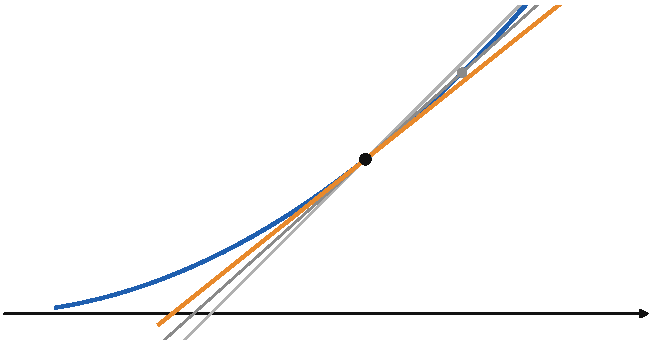
\includegraphics[width=\linewidth]{figures/sieczne.pdf}
\sidecaption{Pochodna jako granica nachyleń. Funkcja $x^2$ (niebieska) i sieczne (szare) przez punkt $(3,9)$ (czarny) i punkty
oddalone o $h=1{,}5$ oraz $0{,}75$. Gdy $h\to0$, sieczna dąży do stycznej (pomarańczowa) o nachyleniu $f'(3)=6$. \label{rys:sieczne}}
\end{figure}

\begin{intuicja}
Pochodna odpowiada na pytanie: „o ile zmieni się wynik, jeśli wejście poruszę o drobinę?”. Zmiana wyniku $\approx f'(x)\cdot$ zmiana wejścia.
To przybliżenie liniowe jest sercem uczenia: nie trzeba znać całej funkcji, wystarczy jej lokalne nachylenie.
\end{intuicja}

Zbierzmy reguły, których użyjemy (pierwsze dwie wynikają wprost z def.~\ref{def:pochodna}):
$(af+bg)'=af'+bg'$, $(fg)'=f'g+fg'$. Najważniejsza jest trzecia.

\begin{twierdzenie}[Reguła łańcuchowa]\label{tw:lancuchowa}
Jeśli $g$ jest różniczkowalna w $x$, a $f$ w $u=g(x)$, to $(f\circ g)'(x)=f'(g(x))\cdot g'(x)$.
\end{twierdzenie}
\begin{pomyslDowodu}
Przybliżamy $g$ prostą o nachyleniu $g'(x)$, a potem $f$ prostą o nachyleniu $f'(u)$. Nachylenia mnożą się.
\end{pomyslDowodu}
\begin{proof}
Różniczkowalność $g$ w $x$ oznacza $g(x+h)-g(x)=g'(x)h+\varepsilon_1(h)h$, gdzie $\varepsilon_1(h)\to0$ przy $h\to0$. Podobnie dla $f$ w $u=g(x)$ i $k=g(x+h)-g(x)$:
$f(u+k)-f(u)=f'(u)k+\varepsilon_2(k)k$, $\varepsilon_2(k)\to0$ przy $k\to0$ (ustalamy $\varepsilon_2(0)=0$). Zatem
\begin{align*}
\frac{f(g(x+h))-f(g(x))}{h} &= \frac{f'(u)\,k+\varepsilon_2(k)\,k}{h} && \pow{(rozwinięcie $f$)}\\
 &= \big(f'(u)+\varepsilon_2(k)\big)\cdot\frac{k}{h} && \pow{(wyłączenie $k$)}\\
 &= \big(f'(u)+\varepsilon_2(k)\big)\big(g'(x)+\varepsilon_1(h)\big). && \pow{($k/h$ z rozwinięcia $g$)}
\end{align*}
Gdy $h\to0$, to $k\to0$ (bo $g$ jest ciągła), więc $\varepsilon_1,\varepsilon_2\to0$ i całość dąży do $f'(u)g'(x)$. To kończy dowód.
\end{proof}

W zwykłym języku: pochodna złożenia to iloczyn pochodnych kolejnych etapów. Sieć neuronowa to długie złożenie, więc jej pochodna to długi iloczyn.

\begin{twierdzenie}[Pochodna sigmoidy]\label{tw:pochodna-sigmoidy}
Funkcja $\sigma(z)=\dfrac{1}{1+e^{-z}}$ spełnia $\sigma'(z)=\sigma(z)\big(1-\sigma(z)\big)$.
\end{twierdzenie}
\begin{pomyslDowodu}
Zapisujemy $\sigma=(1+e^{-z})^{-1}$ i stosujemy regułę łańcuchową.
\end{pomyslDowodu}
\begin{proof}
Niech $u=1+e^{-z}$, więc $\sigma=u^{-1}$, $\dfrac{d\sigma}{du}=-u^{-2}$ i $\dfrac{du}{dz}=-e^{-z}$. Z tw.~\ref{tw:lancuchowa}:
\begin{align*}
\sigma'(z) &= -u^{-2}\cdot(-e^{-z})=\frac{e^{-z}}{(1+e^{-z})^2} && \pow{(reguła łańcuchowa)}\\
 &= \frac{1}{1+e^{-z}}\cdot\frac{e^{-z}}{1+e^{-z}} && \pow{(rozbicie)}\\
 &= \sigma(z)\Big(1-\frac{1}{1+e^{-z}}\Big)=\sigma(z)\big(1-\sigma(z)\big). && \pow{($\tfrac{e^{-z}}{1+e^{-z}}=1-\sigma$)}
\end{align*}
Pochodną można więc policzyć z samej wartości $\sigma$, bez ponownego liczenia wykładnika. To kończy dowód.
\end{proof}

Największa pochodna wynosi $\sigma'(0)=\tfrac12\cdot\tfrac12=\tfrac14$; dla $|z|$ dużego pochodna dąży do zera
(\emph{nasycenie}) --- to jedna z przyczyn, dla których głębokie sieci z samymi sigmoidami uczą się wolno.

\section{Gradient i spadek gradientu}

\haslo{gradient}
\begin{definicja}[Pochodna cząstkowa i gradient]\label{def:gradient}
Dla $f\colon\R^n\to\R$ \emph{pochodna cząstkowa} $\partial f/\partial x_i$ to pochodna po $x_i$ przy pozostałych współrzędnych
traktowanych jak stałe. \emph{Gradient} to wektor tych pochodnych:
$\nabla f(\vect x)=\big(\tfrac{\partial f}{\partial x_1},\dots,\tfrac{\partial f}{\partial x_n}\big)$.
\end{definicja}

\begin{przyklad}\label{prz:gradient}
Dla $f(x,y)=x^2+3xy$: $\partial f/\partial x=2x+3y$, $\partial f/\partial y=3x$. W punkcie $(1,2)$ gradient to $(8,3)$
o długości $\sqrt{73}\approx8{,}54$. Zwiększenie $x$ o $0{,}01$ zwiększa $f$ o ok.\ $0{,}08$, zwiększenie $y$ o $0{,}01$ o ok.\ $0{,}03$.
\end{przyklad}

\begin{twierdzenie}[Gradient wskazuje kierunek najszybszego wzrostu]\label{tw:gradient-najszybszy}
Niech $f$ będzie różniczkowalna w $\vect x$ i $\nabla f(\vect x)\neq\vect0$. Wśród wektorów jednostkowych $\vect d$ pochodna kierunkowa
$\frac{d}{dt}f(\vect x+t\vect d)\big|_{t=0}$ jest największa dla $\vect d=\nabla f/\norm{\nabla f}$ i wynosi wtedy $\norm{\nabla f}$.
\end{twierdzenie}
\begin{pomyslDowodu}
Reguła łańcuchowa zamienia pochodną kierunkową na iloczyn skalarny $\ip{\nabla f}{\vect d}$, a tu działa nierówność Cauchy'ego--Schwarza (tw.~\ref{tw:cs}).
\end{pomyslDowodu}
\begin{proof}
Niech $\phi(t)=f(\vect x+t\vect d)$. Z reguły łańcuchowej dla wielu zmiennych (każda współrzędna zależy od $t$ z pochodną $d_i$):
\begin{align*}
\phi'(0) &= \sum_{i=1}^{n}\frac{\partial f}{\partial x_i}\,d_i && \pow{(reguła łańcuchowa)}\\
 &= \ip{\nabla f(\vect x)}{\vect d}\le\norm{\nabla f}\,\norm{\vect d}=\norm{\nabla f}. && \pow{(tw.~\ref{tw:cs}, $\norm{\vect d}=1$)}
\end{align*}
Równość w Cauchy'ego--Schwarza zachodzi, gdy $\vect d$ jest równoległy do $\nabla f$, czyli $\vect d=\nabla f/\norm{\nabla f}$ (dodatnia wielokrotność, żeby wynik był dodatni).
Wtedy $\phi'(0)=\ip{\nabla f}{\nabla f}/\norm{\nabla f}=\norm{\nabla f}$. To kończy dowód.
\end{proof}

W zwykłym języku: stoisz na zboczu i chcesz iść w górę jak najszybciej --- idź wzdłuż gradientu. Chcemy \emph{zmniejszać}
stratę, więc idziemy \emph{przeciwnie}.

\begin{definicja}[Spadek gradientu]\label{def:spadek}
Dla funkcji straty $L(\vect\theta)$ i \emph{kroku uczenia} $\eta>0$ kolejne przybliżenia to
$\vect\theta_{k+1}=\vect\theta_k-\eta\,\nabla L(\vect\theta_k)$.
\end{definicja}

\begin{naliczbach}
Weźmy $L(x,y)=\tfrac12(x^2+10y^2)$, $\nabla L=(x,10y)$ i start $(1,1)$. Dla $\eta=0{,}05$ kolejne punkty to
$(0{,}95;0{,}5)$, $(0{,}902;0{,}25)$, $(0{,}857;0{,}125)$: schodzimy gładko, ale wolno wzdłuż $x$. Dla $\eta=0{,}15$:
$(0{,}85;-0{,}5)$, $(0{,}722;0{,}25)$, $(0{,}614;-0{,}125)$: współrzędna $y$ zmienia znak w każdym kroku
(zygzak) i jest dwa razy mniejsza w kolejnych krokach. Dla $\eta=0{,}21$ zygzak rośnie i metoda się rozbiega
(dlaczego, wyjaśnia tw.~\ref{tw:eta} w rozdziale~\ref{rozdz:optymalizacja}).
\end{naliczbach}

\begin{figure*}[ht]
\centering
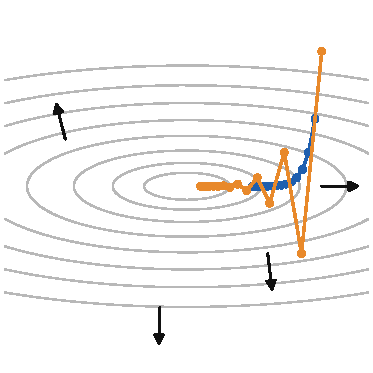
\includegraphics[width=0.88\linewidth]{figures/spadek.pdf}
\caption{Spadek gradientu dla $L=\tfrac12(x^2+10y^2)$ (szare warstwice) z punktu $(1,1)$. Czarne strzałki to gradient w kilku punktach:
zawsze prostopadły do warstwicy i skierowany pod górę, więc krok idzie w przeciwną stronę. Niebieska ścieżka ($\eta=0{,}05$, 14 kroków)
schodzi gładko, ale wolno; pomarańczowa ($\eta=0{,}15$) przeskakuje przez dolinę i zygzakuje. Obie obliczone programem.}
\label{rys:spadek}
\end{figure*}

\section{Propagacja wsteczna na jednym neuronie}

\begin{przyklad}[Gradient strat dla neuronu]\label{prz:backprop}
Neuron: $z=wx+b$, $\hat y=\sigma(z)$, strata $L=(\hat y-y)^2$. Dane: $x=2$, $w=0{,}5$, $b=-0{,}3$, cel $y=1$.
\emph{Przód:} $z=0{,}7$, $\hat y=\sigma(0{,}7)=0{,}6682$, $L=(0{,}6682-1)^2=0{,}1101$.
\emph{Tył} (reguła łańcuchowa, od wyniku ku wejściu):
\begin{align*}
\frac{\partial L}{\partial\hat y} &= 2(\hat y-y)=-0{,}6636,\\
\frac{\partial\hat y}{\partial z} &= \hat y(1-\hat y)=0{,}2217 && \pow{(tw.~\ref{tw:pochodna-sigmoidy})}\\
\frac{\partial L}{\partial w} &= \frac{\partial L}{\partial\hat y}\cdot\frac{\partial\hat y}{\partial z}\cdot\frac{\partial z}{\partial w}
 =(-0{,}6636)(0{,}2217)(2)=-0{,}2943,\\
\frac{\partial L}{\partial b} &= (-0{,}6636)(0{,}2217)(1)=-0{,}1471.
\end{align*}
Sprawdzenie numeryczne: $\big(L(w+10^{-6})-L(w-10^{-6})\big)/(2\cdot10^{-6})=-0{,}2943$. \checkmark
Ujemny gradient oznacza, że \emph{zwiększenie} $w$ zmniejsza stratę: neuron powinien być bardziej pewny odpowiedzi $1$.
\end{przyklad}

\begin{intuicja}
Propagacja wsteczna to reguła łańcuchowa wykonana od końca: zaczynamy od „jak strata zależy od wyniku” i cofając się
przez każdą operację, mnożymy przez jej lokalną pochodną. Każda warstwa musi znać tylko własną pochodną i gradient
przychodzący z góry; dzięki temu da się to zautomatyzować dla dowolnej sieci (PyTorch robi dokładnie to).
\end{intuicja}

\begin{pulapka}
Gradient policzony ręcznie warto \emph{zawsze} porównać z ilorazem różnicowym (jak wyżej). Błąd znaku albo brakującego czynnika
nie powoduje awarii, tylko powolne, dziwne uczenie, które trudno zdiagnozować. Granice stosowalności: różnica $10^{-6}$ w
\texttt{float64} jest dobra; w \texttt{float32} zbyt mały krok tonie w błędach zaokrągleń.
\end{pulapka}

\section*{Podsumowanie}
\begin{itemize}
\item Pochodna to nachylenie stycznej; zmiana wyniku $\approx f'(x)\cdot$ zmiana wejścia.
\item Reguła łańcuchowa: pochodna złożenia to iloczyn pochodnych (tw.~\ref{tw:lancuchowa}); $\sigma'=\sigma(1-\sigma)$.
\item Gradient to wektor pochodnych cząstkowych i wskazuje kierunek najszybszego wzrostu (tw.~\ref{tw:gradient-najszybszy}).
\item Spadek gradientu: $\vect\theta\leftarrow\vect\theta-\eta\nabla L$; za duży krok powoduje zygzak i rozbieżność.
\item Propagacja wsteczna to reguła łańcuchowa liczona od wyniku w stronę wejść; wynik sprawdzamy ilorazem różnicowym.
\end{itemize}

\begin{sprawdz}
\begin{enumerate}
\item Policz pochodną $f(x)=\sigma(3x-1)$ w $x=0$. (Wskazówka: tw.~\ref{tw:lancuchowa} i \ref{tw:pochodna-sigmoidy}.)
\item Dla $f(x,y)=x^2+3xy$ w punkcie $(1,2)$ podaj kierunek jednostkowy najszybszego wzrostu i wartość pochodnej kierunkowej w tym kierunku.
\item Wykonaj jeden krok spadku gradientu z $(1,2)$ dla $L=x^2+3xy$ i $\eta=0{,}01$. O ile (w przybliżeniu) zmieni się $L$?
\item Neuron z przykładu~\ref{prz:backprop} ma $y=0$ zamiast $1$. Jaki jest teraz $\partial L/\partial w$?
\end{enumerate}
\end{sprawdz}

\subsection*{Rozwiązania}
\begin{enumerate}
\item $\sigma(-1)=0{,}2689$, więc $f'(0)=3\sigma(-1)(1-\sigma(-1))=3\cdot0{,}2689\cdot0{,}7311=0{,}590$.
\item $\nabla f=(8,3)$, kierunek $(8,3)/8{,}544=(0{,}936;\,0{,}351)$, pochodna kierunkowa $\norm{\nabla f}=8{,}544$.
\item Krok: $(1,2)-0{,}01(8,3)=(0{,}92;\,1{,}97)$. $L(1,2)=1+6=7$; $L(0{,}92;1{,}97)=0{,}8464+5{,}4372=6{,}2836$. Zmiana $\approx-0{,}716$ (przybliżenie liniowe: $-\eta\norm{\nabla f}^2=-0{,}01\cdot73=-0{,}73$).
\item $\partial L/\partial\hat y=2(0{,}6682-0)=1{,}3364$, więc $\partial L/\partial w=1{,}3364\cdot0{,}2217\cdot2=0{,}5926$ (dodatni: $w$ należy \emph{zmniejszyć}).
\end{enumerate}
